\def\pgfsysdriver{pgfsys-dvisvgm.def}
\documentclass[tikz,border=8pt]{standalone}
\usepackage{amsmath}
% Semantic palette shared by the light and dark exports; geometry and TeX glyphs stay identical.
\ifdefined\FigureDark
  \definecolor{FigureForeground}{HTML}{E1E8DF}
  \definecolor{FigureMuted}{HTML}{94A69B}
  \definecolor{FigureBlue}{HTML}{8CC5F2}
  \definecolor{FigureOrange}{HTML}{F4B76B}
  \definecolor{FigureRed}{HTML}{F28E86}
  \definecolor{FigureBlueFill}{HTML}{273F4F}
  \definecolor{FigureOrangeFill}{HTML}{4A3726}
  \definecolor{FigurePaper}{HTML}{1B2420}
\else
  \definecolor{FigureForeground}{HTML}{202C29}
  \definecolor{FigureMuted}{HTML}{68766E}
  \definecolor{FigureBlue}{HTML}{245A88}
  \definecolor{FigureOrange}{HTML}{986000}
  \definecolor{FigureRed}{HTML}{A44030}
  \definecolor{FigureBlueFill}{HTML}{E5EDF8}
  \definecolor{FigureOrangeFill}{HTML}{FFF0D8}
  \definecolor{FigurePaper}{HTML}{FBFAF7}
\fi

\usetikzlibrary{arrows.meta,backgrounds}
\colorlet{positive}{FigureBlue}
\colorlet{negative}{FigureRed}
\begin{document}
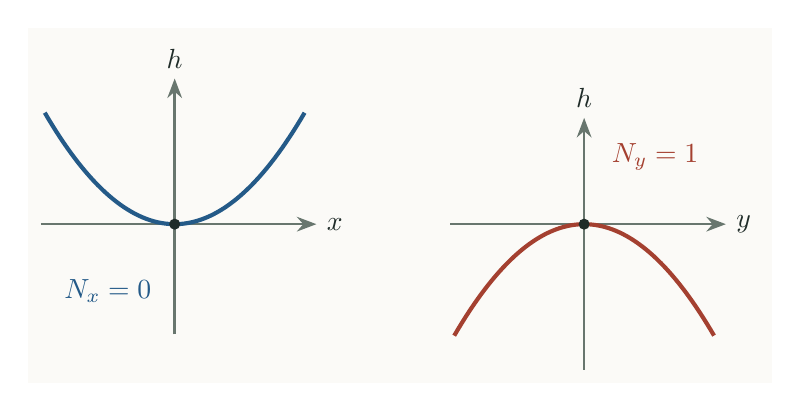
\begin{tikzpicture}[color=FigureForeground,>=Stealth,font=\normalsize,line width=.9pt,background rectangle/.style={fill=FigurePaper},show background rectangle]
  % Two perpendicular one-dimensional sections of h=(x^2-y^2)/2.
  \begin{scope}[xshift=0cm]
    \draw[->,FigureMuted] (-1.7,0)--(1.8,0) node[right,FigureForeground] {$x$};
    \draw[->,FigureMuted] (0,-1.4)--(0,1.85) node[above,FigureForeground] {$h$};
    \draw[positive,line width=1.5pt,domain=-1.65:1.65,samples=70]
      plot (\x,{.52*\x*\x});
    \fill (0,0) circle (2pt);
    \node[positive] at (-.85,-.85) {$N_x=0$};
  \end{scope}
  \begin{scope}[xshift=5.2cm]
    \draw[->,FigureMuted] (-1.7,0)--(1.8,0) node[right,FigureForeground] {$y$};
    \draw[->,FigureMuted] (0,-1.85)--(0,1.35) node[above,FigureForeground] {$h$};
    \draw[negative,line width=1.5pt,domain=-1.65:1.65,samples=70]
      plot (\x,{-.52*\x*\x});
    \fill (0,0) circle (2pt);
    \node[negative] at (.90,.85) {$N_y=1$};
  \end{scope}
\end{tikzpicture}
\end{document}
